\documentclass[11pt]{article}

\usepackage[margin=1in]{geometry}
\usepackage{amsmath,amssymb,amsthm}
\usepackage[T1]{fontenc}
\usepackage[utf8]{inputenc}
\usepackage{lmodern}
\usepackage{microtype}
\usepackage{booktabs}
\usepackage{longtable}
\usepackage[hidelinks]{hyperref}
\usepackage{parskip}
\usepackage{tikz}
\usetikzlibrary{positioning}

% No section numbering in subsection references but keep numbering
\setcounter{secnumdepth}{3}

\title{The Logical Geography of Mathematical Physics:\\
Constructive Calibration from Density Matrices\\to the Born Rule\\[1em]
\large A Companion to the Constructive Calibration Programme (Paper~10, v2.0)}
\author{Paul Chun-Kit Lee\\New York University}
\date{February 2026}

\begin{document}
\maketitle

\begin{abstract}
This paper synthesizes the machine-verified results of the author's constructive calibration programme --- spanning functional analysis (Papers~2, 7), quantum spectra (Paper~4), uncertainty relations (Paper~6), statistical mechanics (Papers~8, 9), quantum information (Paper~11), general relativity (Paper~13), quantum decoherence (Paper~14), conservation laws (Paper~15), and quantum measurement statistics (Paper~16) --- into a single interpretive framework. It contains no new theorems or formalizations. Its purpose is to assemble the calibration table, establish the certification methodology, formulate a working hypothesis, and pose a research program.

The calibration table now contains twenty-five entries spanning BISH to undecidable, populated by machine-verified Lean~4 formalizations totalling approximately 12,000 lines of code across six domains of mathematical physics. The results establish that preparation uncertainty, finite-size approximations, quantum entanglement structure (Tsirelson bound, Bell state entropy, partial trace), Schwarzschild interior finite-time physics, finite-step decoherence bounds, local conservation laws, and Born probabilities are fully constructive (BISH); that measurement uncertainty, locale spatiality, and the strong law of large numbers require Dependent Choice (DC$_\omega$); that exact spectral membership requires Markov's Principle (MP, on an orthogonal axis); that singular states and the bidual gap require WLPO; and that the thermodynamic limit, geodesic incompleteness, exact decoherence, and global energy existence require exactly LPO via bounded monotone convergence. The logical strength required correlates systematically with the degree of physical idealization, and the same BMC~$\equiv$~LPO equivalence now governs completed limits in four independent domains --- statistical mechanics, general relativity, quantum decoherence, and conservation laws --- a domain invariance that substantially strengthens the evidence that the costs are intrinsic to the physics.

We establish a certification methodology with three levels --- mechanically certified, structurally verified, and intentional classical content --- that addresses the relationship between Lean~4's classical metatheory (Mathlib) and the series' constructive claims. We formulate a working hypothesis: all non-constructive costs arise from infinite-dimensional idealization layers, not from finite-dimensional or finite-time physical content. We present formulation-invariance evidence (Papers~8, 9) and domain-invariance evidence (Papers~8, 13, 14, 15), distinguish this position from operationalism, and situate the proposal within the broader landscape of constructive approaches to physics.
\end{abstract}

\section{Introduction}

Mathematical physics is written in the language of classical mathematics. Physicists invoke the law of excluded middle, the axiom of choice, and the full strength of Zermelo-Fraenkel set theory without hesitation, and the resulting formalism produces spectacularly accurate predictions. The question of whether this logical strength is \emph{necessary} --- whether the same physical content could be extracted from weaker principles --- has been raised periodically since Brouwer, but has remained largely a philosophical curiosity. The practical success of classical mathematics leaves little incentive to investigate constructive alternatives.

This paper argues that the question deserves revival, and that recent machine-verified results in constructive reverse mathematics provide the tools to address it with unprecedented precision. The central observation is simple: when one examines the standard mathematical infrastructure of quantum statistical mechanics through a constructive lens, the logical principles required at each level of idealization fall into a structured hierarchy --- predominantly a linear chain, but with orthogonal axes --- that correlates with the degree of physical abstraction.

\textbf{Scope and status.} This paper contains no new proofs or formalizations. All formal results are machine-verified in the eleven companion papers [Lee 2026a, 2026b, 2026c, 2026e, 2026f, 2026g, 2026h, 2026i, 2026j, 2026k, 2026l]. Our contribution here is interpretive: we assemble the verified results into a calibration table mapping layers of mathematical physics to positions in the constructive hierarchy, formulate a working hypothesis about what this mapping means, establish the series-wide certification methodology, and report the outcome of formulation-invariance and domain-invariance tests. Papers~2, 6, 7, 8, 9, 11, 13, 14, 15, and~16 employ constructive reverse mathematics (CRM) over Mathlib-based Lean~4 formalizations; Paper~4 employs the Axiom Calibration (AxCal) framework in mathlib-free Lean~4. Paper~16's DC$_\omega$ layer is axiomatised following the same interface-axiom methodology as the BMC~$\leftrightarrow$~LPO equivalence in Papers~8, 13, 14, and~15. The calibration results from both methodologies are compatible and jointly populate the table below.
\textbf{The calibration table.} The following table summarizes the current state of the programme. Each row assigns to a layer of mathematical physics the constructive omniscience principle required for its standard formulation, together with the verification status. We maintain a distinction between two levels of evidence:

\begin{itemize}
\item \textbf{Calibrated}: a verified equivalence or tight bound --- the physical statement is provably equivalent to ($\equiv$) or bounded by ($\leq$) the corresponding principle over BISH, with both directions machine-checked.
\item \textbf{Route-costed}: the logical cost of a \emph{standard proof route} has been identified, but minimality has not been established --- a lower-cost alternative route has not been ruled out.
\end{itemize}

All entries below are calibrated unless otherwise noted. Entries marked ``$\leq$'' indicate an upper bound (the physical statement has been shown to require \emph{at most} the stated principle, but the exact cost may be lower):

\begin{center}
\begin{longtable}{@{}p{5.2cm}lll@{}}
\toprule
Layer & Principle & Status & Source \\
\midrule
\endfirsthead
\toprule
Layer & Principle & Status & Source \\
\midrule
\endhead
Finite-volume physics & BISH & Calibrated & Trivial \\
Finite-size approximations & BISH & Calibrated & Papers 8, 9 (Part~A) \\
Finite spectral approximations & BISH & Calibrated & Paper 4 (S0, S4)$^\dagger$ \\
Preparation uncertainty (HUP) & BISH & Calibrated & Paper 6 \\
$S_1(H)$ non-reflexivity ($\neg$-form) & BISH & Calibrated & Paper 7 \\
Measurement uncertainty (HUP) & $\leq$ DC$_\omega$ & Calibrated & Paper 6 \\
Locale spatiality (separable) & DC$_\omega$ & Calibrated & Paper 4 (S2)$^\dagger$ \\
Frequentist convergence (SLLN) & $\leq$ DC$_\omega$ & Calibrated & Paper 16 \\
Exact spectral membership & MP & Calibrated & Paper 4 (S1)$^\dagger$ \\
Spectral separation (non-sep.) & WLPO & Calibrated & Paper 4 (S3, via Paper~2)$^\dagger$ \\
Bidual-gap / singular states & $\equiv$ WLPO & Calibrated & Papers 2, 7 \\
Bell nonlocality (CHSH/Tsirelson) & BISH & Calibrated & Paper 11 \\
Entanglement entropy (qubit Bell state) & BISH & Calibrated & Paper 11 \\
Partial trace (finite-dim) & BISH & Calibrated & Paper 11 \\
Schwarzschild interior (finite-time) & BISH & Calibrated & Paper 13 \\
Finite-step decoherence bounds & BISH & Calibrated & Paper 14 \\
Local conservation (Noether) & BISH & Calibrated & Paper 15 \\
Finite-volume conserved charge & BISH & Calibrated & Paper 15 \\
Born probability (finite-dim) & BISH & Calibrated & Paper 16 \\
Chebyshev bound (weak law) & BISH & Calibrated & Paper 16 \\
Thermodynamic limit existence & $\equiv$ LPO & Calibrated & Papers 8, 9 (Part~B) \\
Geodesic incompleteness (completed limit) & $\equiv$ LPO & Calibrated & Paper 13 \\
Exact decoherence (wave fn collapse) & $\equiv$ LPO & Calibrated & Paper 14 \\
Global energy (infinite-volume) & $\equiv$ LPO & Calibrated & Paper 15 \\
Spectral gap decidability & Undecidable & Established & Cubitt et al.\ 2015 \\
\bottomrule
\end{longtable}
\end{center}

\begin{figure}[ht]
\centering
\resizebox{\textwidth}{!}{%
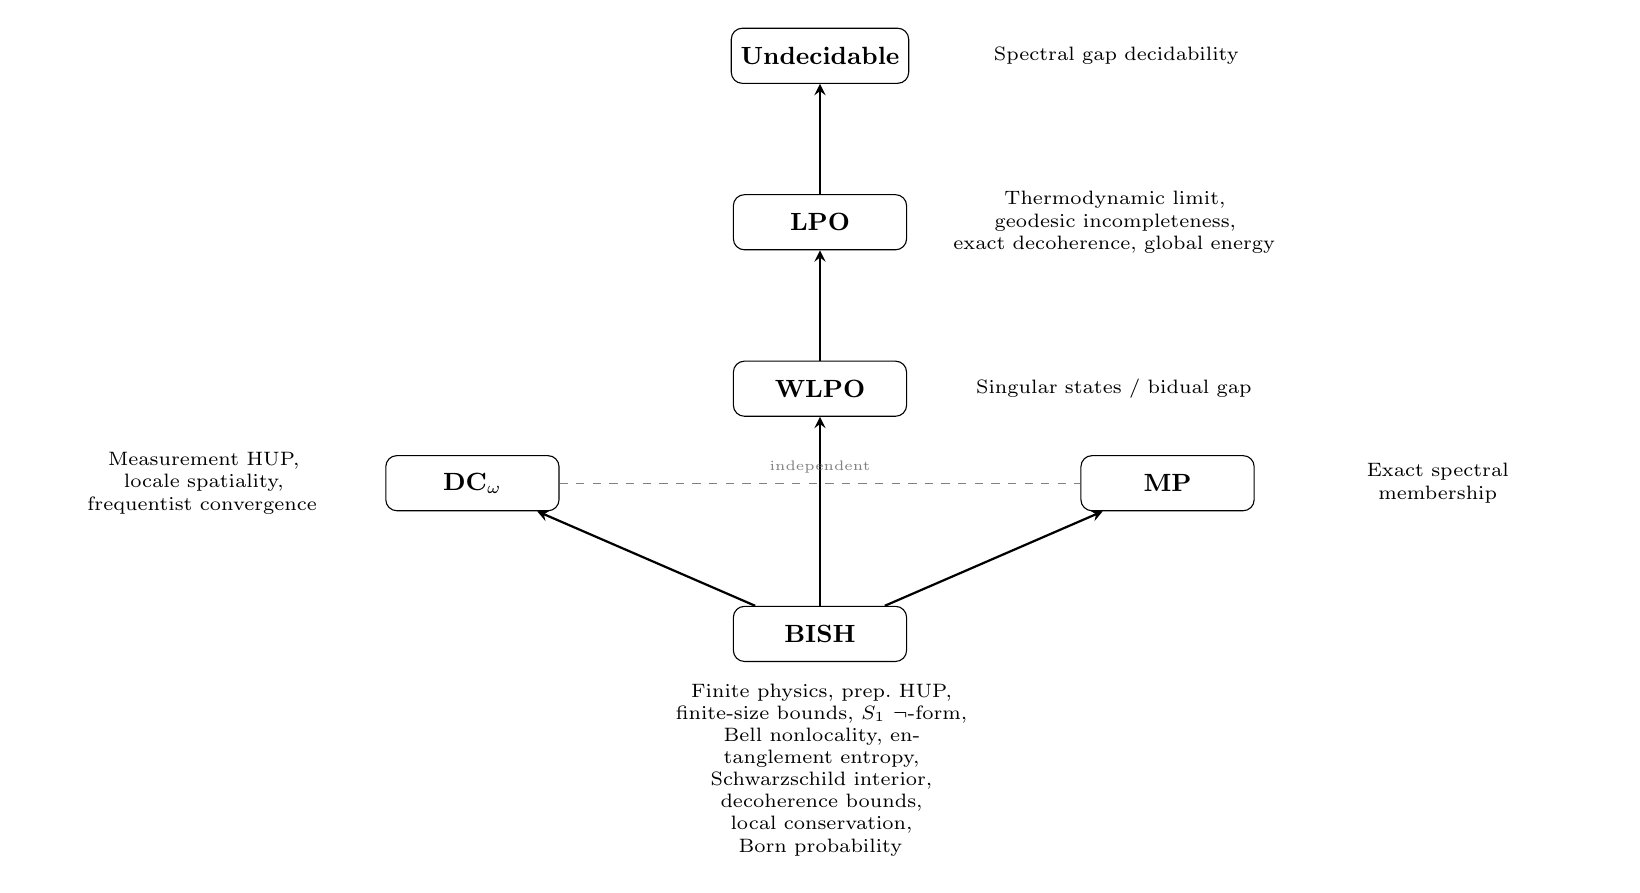
\begin{tikzpicture}[
  node distance=1.4cm and 2.8cm,
  principle/.style={draw, rounded corners, minimum width=2.2cm, minimum height=0.7cm, font=\small\bfseries},
  physlabel/.style={font=\scriptsize, text width=4.2cm, align=center},
  >=stealth
]
% Main spine
\node[principle] (bish) {BISH};
\node[principle, above=2.4cm of bish] (wlpo) {WLPO};
\node[principle, above=of wlpo] (lpo) {LPO};
\node[principle, above=of lpo] (undec) {Undecidable};

% Orthogonal branches
\node[principle, above left=1.2cm and 2.2cm of bish] (dc) {DC$_\omega$};
\node[principle, above right=1.2cm and 2.2cm of bish] (mp) {MP};

% Edges (Hasse diagram: only covering relations)
\draw[thick, ->] (bish) -- (dc);
\draw[thick, ->] (bish) -- (mp);
\draw[thick, ->] (bish) -- (wlpo);
\draw[thick, ->] (wlpo) -- (lpo);
\draw[thick, ->] (lpo) -- (undec);

% Physical labels
\node[physlabel, below=0.15cm of bish] {Finite physics, prep.\ HUP,\\finite-size bounds, $S_1$ $\neg$-form,\\Bell nonlocality, entanglement entropy,\\Schwarzschild interior, decoherence bounds,\\local conservation, Born probability};
\node[physlabel, left=0.1cm of dc] {Measurement HUP,\\locale spatiality,\\frequentist convergence};
\node[physlabel, right=0.1cm of mp] {Exact spectral\\membership};
\node[physlabel, right=0.4cm of wlpo] {\scriptsize Singular states / bidual gap};
\node[physlabel, right=0.4cm of lpo] {\scriptsize Thermodynamic limit,\\geodesic incompleteness,\\exact decoherence, global energy};
\node[physlabel, right=0.4cm of undec] {\scriptsize Spectral gap decidability};

% Orthogonality annotation
\draw[dashed, gray] (dc) -- node[above, font=\tiny, gray] {independent} (mp);

\end{tikzpicture}%
}
\caption{The logical geography of mathematical physics. Arrows indicate strict implication over BISH. The omniscience spine (BISH $<$ WLPO $<$ LPO) forms the dominant vertical chain. DC$_\omega$ and MP occupy orthogonal positions: neither implies the other, neither implies WLPO, and WLPO implies neither. LPO implies both WLPO and MP but is independent of DC$_\omega$, which is a choice principle rather than an omniscience principle. Physical layers are annotated with their calibrated logical cost.}
\label{fig:geography}
\end{figure}

\noindent$^\dagger$AxCal methodology --- assembly proof verified in Lean, mathematical prerequisites axiomatized as bridge lemmas. See \S\ref{sec:machine}. Paper~6 v2 has been upgraded to CRM (Mathlib-based) and no longer carries this designation.

\textbf{New entries in v1.1.} Paper~11 extends the calibration from ``states, limits, spectra'' to ``tensor products, entanglement, correlations.'' The BISH results confirm that quantum compositional structure --- the infrastructure of entanglement itself --- carries no non-constructive cost. All costs in quantum theory arise from infinite-dimensional limits, not from the algebraic structure of quantum mechanics. Paper~13 extends from statistical mechanics to gravitation. The Schwarzschild interior's finite-time physics (cycloid geodesics, Kretschner scalar divergence) is BISH, while geodesic incompleteness --- asserting the limit of proper time along the infalling trajectory as a completed real number --- costs exactly LPO via bounded monotone convergence, mirroring Paper~8's thermodynamic limit. The event horizon thus functions as a \emph{logical boundary}: the same BMC~$\equiv$~LPO equivalence that separates finite-volume from infinite-volume physics in statistical mechanics separates finite-time from completed-limit physics in general relativity.

\textbf{New entries in v2.0.} Papers~14, 15, and~16 extend the calibration to three further domains. Paper~14 [Lee 2026j] calibrates quantum decoherence: finite-step decoherence bounds (geometric decay of off-diagonal coherence) are BISH, while exact decoherence --- the completed-limit formulation of wave function collapse --- costs LPO via the Antitone Bounded Convergence (ABC) equivalence, fully proved equivalent to BMC in Lean with no custom axioms. This is the third BMC~$\equiv$~LPO domain after Papers~8 and~13. Paper~15 [Lee 2026k] calibrates Noether's theorem and global conservation laws: local conservation and finite-volume conserved charge are BISH, while global energy existence --- for systems with non-negative energy density --- costs LPO via Nonneg\-ative Partial Sum Convergence (NPSC), again fully proved equivalent to BMC in Lean. This is the fourth BMC~$\equiv$~LPO domain and the first calibration of a structural law rather than a physical prediction. Notably, the sign of the conserved density is logically significant: energy (non-negative) gives monotone partial sums fitting BMC, while charge (signed) gives oscillatory partial sums that do not. Paper~16 [Lee 2026l] calibrates the Born rule: Born probabilities, expectation reality, variance, and the Chebyshev bound are all BISH, while the strong law of large numbers (frequentist convergence) requires DC$_\omega$. Paper~16 is a technical note whose contribution is programme completeness --- populating the DC$_\omega$ axis with physical content from quantum measurement statistics --- rather than mathematical novelty. Together, these three papers double the BMC~$\equiv$~LPO domain-invariance evidence from two to four instances and populate the DC$_\omega$ axis alongside Papers~4 and~6.

For the thermodynamic limit, the calibration has been verified across two independent mathematical formulations (transfer-matrix and combinatorial), establishing formulation-invariance [Lee 2026e]. The principal progression from BISH through WLPO, LPO, to undecidability is monotone in the degree of physical idealization: each step moves further from what a finite laboratory can instantiate. However, the table also reveals an orthogonal axis: Markov's Principle (MP), required for exact spectral membership (Paper~4), is independent of WLPO --- neither implies the other over BISH. The logical geography of physics is thus a partial order rather than a simple linear chain, with the omniscience hierarchy (BISH $<$ WLPO $<$ LPO $<$ LEM) as its dominant spine and choice/decidability principles (DC$_\omega$, MP) providing lateral dimensions.

\section{Background: Constructive Reverse Mathematics}

\subsection{The constructive hierarchy}

Bishop-style constructive mathematics (BISH) is mathematics carried out with intuitionistic logic and dependent choice, but without the law of excluded middle (LEM), the full axiom of choice, or any continuity principles. It is a common core: every BISH theorem is valid in classical mathematics, in recursive mathematics, and in Brouwerian intuitionism. The constructive hierarchy consists of principles that extend BISH by calibrated amounts:

\textbf{WLPO} (Weak Limited Principle of Omniscience): For any binary sequence $\alpha : \mathbb{N} \to \{0,1\}$, either $(\forall n)(\alpha(n) = 0)$ or $\neg(\forall n)(\alpha(n) = 0)$. This is the weakest standard omniscience principle. It asserts that ``all zeros'' is decidable --- not by producing a counterexample, but by deciding whether one exists.

\textbf{LPO} (Limited Principle of Omniscience): For any binary sequence $\alpha : \mathbb{N} \to \{0,1\}$, either $(\forall n)(\alpha(n) = 0)$ or $(\exists n)(\alpha(n) = 1)$. This is strictly stronger than WLPO. It asserts that a binary sequence either is identically zero or has a term equal to one --- a genuine dichotomy, not merely the negation of universality.

\textbf{LEM} (Law of Excluded Middle): For any proposition $P$, either $P$ or $\neg P$. Full classical logic.

The strict implications are: BISH $<$ WLPO $<$ LPO $<$ LEM. Each inclusion is proper: there exist models of BISH + WLPO in which LPO fails, and models of BISH + LPO in which LEM fails.

These principles have a precise proof-theoretic location. Both WLPO and LPO require $\Sigma^0_1$ excluded middle (decidability of existential arithmetic statements), while full LEM requires excluded middle at all arithmetic levels. The omniscience hierarchy thus decomposes a specific fragment of the gap between intuitionistic and classical arithmetic.

\subsection{The methodology: constructive reverse mathematics}

Classical reverse mathematics (Friedman, Simpson) asks: which set-existence axioms are needed to prove the theorems of ordinary mathematics? The base theory is RCA$_0$ (recursive comprehension), and the programme classifies theorems by their equivalence to one of five standard systems.

Constructive reverse mathematics (CRM) asks the analogous question over BISH: which omniscience principles are needed? A CRM result takes the form ``Theorem~$T$ is equivalent to principle~$P$ over BISH,'' meaning (i) BISH + $P$ proves $T$, and (ii) BISH + $T$ proves $P$. The equivalence is proven in a classical metatheory --- this is essential and not a defect, just as Simpson's results are proven in ZFC. The meta-classical reasoning is quarantined: it establishes that the object-level equivalence holds, without contaminating the constructive content.

The programme was initiated by Ishihara [1992, 2006] and developed by Bridges and V\^{\i}\c{t}\u{a} [2006], among others. Key results include the equivalence of LPO with bounded monotone convergence, of WLPO with the existence of infima of bounded sequences, and the Ishihara trichotomy relating WLPO to the sequential structure of Banach spaces.

\subsection{Machine verification}\label{sec:machine}

A distinctive feature of this programme is its reliance on formal verification in Lean~4. The companion papers provide complete Lean formalizations: approximately 5,500 lines for the bidual gap equivalence (Paper~2), 759 lines across 8 modules for the physical bidual gap (Paper~7), 1,374 lines across 18 modules for the 1D Ising transfer-matrix formalization (Paper~8), 1,319 lines across 18 modules for the independent combinatorial formalization (Paper~9), over 700 lines for the quantum spectra calibration (Paper~4, AxCal), approximately 420 lines across 4 modules for the Heisenberg uncertainty principle (Paper~6 v2), 639 lines across 8 modules for the Tsirelson bound and Bell state entropy (Paper~11), 1,021 lines across 8 modules for Schwarzschild geodesic incompleteness (Paper~13), 805 lines across 9 modules for quantum decoherence (Paper~14), approximately 520 lines across 6 modules for Noether's theorem and global energy (Paper~15), and 564 lines across 9 modules for the Born rule and measurement statistics (Paper~16). The \texttt{\#print axioms} command provides a machine-checkable certificate that a given proof uses no classical axioms beyond those explicitly declared --- a level of assurance unavailable to pen-and-paper proofs about constructive validity. For a systematic treatment of the relationship between this classical certificate and the series' constructive claims, see \S\ref{sec:methodology}.

\textbf{Methodological distinction.} The companion papers employ two distinct formalization methodologies. Papers~2, 6, 7, 8, 9, 11, 13, 14, 15, and~16 use \emph{constructive reverse mathematics (CRM)} over Mathlib: theorems are proved from Mathlib's library of formalized mathematics, and \texttt{\#print axioms} certificates verify that no classical axioms beyond those explicitly declared appear in the proof term. These are deep formalizations --- the mathematical content is machine-checked end-to-end. Paper~6 was originally formalized in the AxCal framework (v1, ${\sim}960$ lines) and subsequently upgraded to a full CRM formalization over Mathlib (v2, ${\sim}420$ lines), with all mathematical prerequisites (Cauchy-Schwarz inequality, inner product space algebra, self-adjoint operator properties) derived from Mathlib rather than axiomatized. Paper~16 uses CRM over Mathlib for the BISH content, with the DC$_\omega$ layer axiomatised following the same interface-axiom methodology as the BMC~$\leftrightarrow$~LPO equivalence in Papers~8, 13, 14, and~15. Paper~4 uses the \emph{Axiom Calibration (AxCal)} framework in mathlib-free Lean~4: mathematical prerequisites are axiomatized as unproven bridge lemmas, and Lean verifies that the \emph{assembly} of these prerequisites into the target theorem is logically valid and constructive. AxCal formalizations verify the logical architecture of a proof --- which principles are needed at the assembly level --- but delegate the verification of mathematical prerequisites to the axiom layer. The calibration claims from both methodologies populate the table below; the distinction in verification depth should be understood when interpreting the entries.

\section{Methodology: Formalization in a Classical Metatheory}\label{sec:methodology}

\subsection{The standard CRM methodology}

Constructive reverse mathematics has always operated within a classical metatheory. Bridges and Richman prove their equivalences using informal mathematics that implicitly includes excluded middle at the meta-level. Ishihara works in classical set theory. Simpson's \emph{Subsystems of Second-Order Arithmetic} uses ZFC as the metatheory for reverse mathematics over RCA$_0$. The question is never whether the metatheory is constructive; it is always whether the \emph{object-level theorem} can be stated and proved using only the principles under investigation.

This paper's companion formalizations (Papers~1--9, 11, 13) adopt the same methodology in a mechanized setting. Lean~4 with Mathlib is the classical metatheory. The constructive content is extracted by inspecting what the proofs actually use, as reported by \texttt{\#print axioms}.

\subsection{Three certification levels}

The formalizations in this series achieve different levels of certification for their constructive claims:

\begin{enumerate}
\item \textbf{Mechanically certified.} The Lean build target compiles without \texttt{Classical.choice} in the \texttt{\#print axioms} output. Constructive purity is verified by the machine itself. Examples: Paper~2's P2\_Minimal and Paper~7's P7\_Minimal --- dependency-free Lean build targets that certify the core equivalences without any Mathlib imports.

\item \textbf{Structurally verified.} The Lean build target compiles with \texttt{Classical.choice} inherited from Mathlib's typeclass infrastructure, but the proof structure uses only constructively valid reasoning (finite-dimensional algebra, explicit computation, Hahn-Banach for separable spaces). The BISH claim is established by mathematical argument about proof content, supported by the machine-checked proof structure. Examples: Papers~7 (P7\_Full), 8A, 9A, 11, and the BISH content of Paper~13.

\item \textbf{Intentional classical content.} The proof uses classical principles by design --- the classical content is the \emph{theorem}, not an artifact of the library. \texttt{\#print axioms} correctly reports classical axioms because the theorem \emph{requires} them. Examples: Paper~8B (LPO appears because BMC~$\equiv$~LPO is the theorem), Paper~13's main theorem (LPO equivalence is the result), Paper~7's reverse direction (WLPO appears as a hypothesis).
\end{enumerate}

\subsection{The Mathlib question}

Why does \texttt{Classical.choice} appear in proofs about finite matrices (Paper~11) or explicit trigonometric computations (Paper~13's cycloid)?

Mathlib imports \texttt{Classical.em} and \texttt{Classical.choice} at the library level. These enter the axiom profile through typeclass resolution --- when Lean resolves \texttt{Decidable} instances for $\mathbb{R}$, $\mathbb{C}$, or matrix entries, it traces through classical infrastructure regardless of whether the proof term actually uses decidability. The result: \texttt{\#print axioms} cannot distinguish between ``this theorem requires classical logic'' and ``this theorem's proof happens to be written in a library that assumes classical logic.''

This is not a defect. It is the expected behavior of a classical metatheory. Just as Bridges and Richman's informal proofs do not mechanically certify BISH by virtue of being written in English, Lean proofs do not mechanically certify BISH by virtue of compiling. What the Lean proofs provide is something informal proofs cannot: a machine-checked guarantee that every step type-checks, that no implicit gaps exist, and that axiom dependencies are exhaustively reported.

\subsection{The role of minimal artifacts}

Where the constructive claim is non-trivial or the proof involves genuine logical content, the series provides dependency-free ``minimal'' artifacts. These are separate Lean build targets that axiomatize Mathlib-dependent results and verify the logical reduction chain without classical imports.

\begin{center}
\begin{tabular}{@{}llll@{}}
\toprule
Paper & Full Artifact & Minimal Artifact & Certification \\
\midrule
2 & P2\_Full (Mathlib, 3100 lines) & P2\_Minimal (dep-free, $\sim$200 lines) & Mechanically certified \\
7 & P7\_Full (Mathlib, 754 lines) & P7\_Minimal (dep-free, 277 lines) & Mechanically certified \\
8A & Transfer matrix (BISH) & --- & Structurally verified \\
8B & BMC $\leftrightarrow$ LPO & --- & Intentional classical \\
9 & Combinatorial Ising & --- & Structurally verified \\
11 & Tsirelson + Bell (639 lines) & --- & Structurally verified \\
13 (BISH) & Cycloid, Kretschner (128 lines) & --- & Structurally verified \\
13 (LPO) & Main theorem (1021 lines) & --- & Intentional classical \\
14 (BISH) & Decoherence bounds (805 lines) & --- & Structurally verified \\
14 (LPO) & Exact decoherence (805 lines) & --- & Intentional classical \\
15 (BISH) & Noether, finite energy ($\sim$520 lines) & --- & Structurally verified \\
15 (LPO) & Global energy ($\sim$520 lines) & --- & Intentional classical \\
16 (BISH) & Born probability, weak law (564 lines) & --- & Structurally verified \\
16 (DC$_\omega$) & SLLN (564 lines) & --- & Intentional classical \\
\bottomrule
\end{tabular}
\end{center}

No minimal artifact is needed for Papers~11, 13, 14, 15, or~16's BISH content: finite-dimensional matrix algebra (Papers~11, 14, 16), explicit trigonometric evaluation (Paper~13), and finite-sum manipulation (Paper~15) being BISH is uncontroversial. The minimal artifacts are reserved for cases where the logical architecture itself is substantive (Papers~2 and~7).

\subsection{Limitations}

A fully constructive Lean library for CRM --- separating classical and constructive content at the typeclass level, allowing mechanical BISH certification without dependency-free artifacts --- does not currently exist. Building one is a major infrastructure project beyond this series' scope. The methodology described above is the best available approach given current tooling, and mirrors the standard practice in CRM where the metatheory is classical and the constructive content is established by mathematical argument.

\section{The Verified Results}

We summarize the companion papers that anchor the calibration table.

\subsection{The Bidual Gap equivalence (Paper~2)}

A \emph{bidual-gap witness} for a Banach space $X$ is a constructive datum certifying that the canonical image $J(X)$ is proper in $X^{**}$: an explicit element $\Psi \in X^{**}$ together with a positive separation from $J(X)$ --- that is, an explicit functional and threshold such that $\|\Psi - Jx\| > \delta$ for all $x \in X$.

\textbf{Theorem} [Lee 2026a]. Over BISH, the following are equivalent:

\begin{enumerate}
\item[(i)] WLPO.
\item[(ii)] There exists a Banach space $X$ and a bidual-gap witness for $X$.
\end{enumerate}

The proof proceeds via the Ishihara kernel technique. The forward direction (WLPO $\to$ gap) constructs a concrete non-reflexive space. The reverse direction (gap $\to$ WLPO) extracts an Ishihara kernel from the gap witness and derives WLPO using only intuitionistic logic --- the classical content is quarantined in the kernel extraction. The Lean formalization verifies this separation: \texttt{WLPO\_of\_kernel} carries no classical axioms (the constructive consumer), while \texttt{WLPO\_of\_gap} --- fenced in \texttt{section ClassicalMeta} --- carries \texttt{Classical.choice} through the kernel construction (the classical producer) before delegating to \texttt{WLPO\_of\_kernel}.

This result establishes that non-reflexivity itself --- the mere existence of a Banach space with a bidual gap --- has the exact logical strength of WLPO.

\subsection{The Physical Bidual Gap (Paper~7)}

\textbf{Theorem} [Lee 2026b]. Let $H$ be a separable infinite-dimensional Hilbert space.

\begin{enumerate}
\item[(i)] (Unconditional) $S_1(H)$ is not reflexive: $\neg(J \text{ is surjective})$, provable in BISH without any omniscience principle.
\item[(ii)] (Constructive witness bound) Any bidual-gap witness for $S_1(H)$ --- any constructive datum exhibiting a specific $\Psi \in (S_1(H))^{**}$ separated from $J(S_1(H))$ --- implies WLPO.
\end{enumerate}

This anchors the abstract result of Paper~2 in the canonical state space of quantum mechanics. Density matrices --- the mathematical representatives of quantum states --- are positive trace-class operators of unit trace. The bidual $S_1(H)^{**}$ contains functionals that are not represented by any density matrix. These are the \emph{singular states}: mathematically well-defined objects in the bidual that correspond to no physical preparation procedure. In the language of operator algebras, every state $\omega$ on a von Neumann algebra admits a unique decomposition $\omega = \omega_n + \omega_s$ into normal and singular parts [Takesaki 1979] --- the noncommutative analogue of the Lebesgue decomposition. The singular component $\omega_s$ vanishes on all compact operators, detecting only behavior at spatial infinity.

The crucial distinction is between the \emph{$\neg$-form} and the \emph{witness form}. Statement~(i) --- that $S_1(H)$ is not reflexive --- is a negative result provable in BISH: singular states cannot be ruled out. Statement~(ii) shows that \emph{upgrading} this to a positive witness --- actually exhibiting a singular state with constructive separation data --- requires WLPO. This gap between ``cannot be ruled out'' and ``can be explicitly produced'' is characteristic of constructive mathematics, and it is precisely where the omniscience principle enters: not in the \emph{existence} of singular states, but in \emph{constructively exhibiting} one with separation data.

\subsection{Dispensability of the thermodynamic limit (Paper~8, Part~A)}

\textbf{Theorem} [Lee 2026c, Part~A]. For the one-dimensional Ising model with nearest-neighbour coupling $J$ and inverse temperature $\beta$, the finite-size free energy density $f_N(\beta)$ satisfies:
\[
|f_N(\beta) - f_\infty(\beta)| \leq \frac{1}{N} \cdot \tanh(\beta J)^N
\]

This bound is provable in BISH without any omniscience principle. The proof proceeds via the transfer matrix method: the partition function $Z_N = \operatorname{Tr}(T^N)$ where $T$ is the $2\times 2$ transfer matrix, the eigenvalues $\lambda_+ > \lambda_- > 0$ are constructively computable, and the error bound follows from the ratio $\lambda_-/\lambda_+ = \tanh(\beta J) < 1$. Every step --- eigenvalue computation, logarithmic estimates, the geometric decay --- is valid in BISH.

The significance is not that a direct computation is constructive --- that would be trivially true. The significance is that the \emph{approximation of the infinite-volume answer by finite-system data} is constructively valid, even though the infinite-volume answer itself is defined via a limit whose existence requires LPO. The empirical content of the thermodynamic limit is available without the idealization. Paper~9 [Lee 2026e] independently confirms this result via a purely combinatorial derivation using bond variables and the binomial parity sieve, with no linear algebra.

\subsection{The LPO cost of the thermodynamic limit (Paper~8, Part~B)}

\textbf{Theorem} [Lee 2026c, Part~B]. Over BISH, the following are equivalent:

\begin{enumerate}
\item[(i)] LPO.
\item[(ii)] Every bounded monotone sequence of real numbers converges (BMC).
\end{enumerate}

The equivalence BMC $\Leftrightarrow$ LPO is due to Bridges and V\^{\i}\c{t}\u{a} [2006]. Paper~8 instantiates this equivalence: the free energy densities $f_N(\beta)$ form a bounded monotone sequence (by subadditivity of $\log Z$), and asserting that $f_\infty(\beta) = \lim f_N(\beta)$ \emph{exists as a completed real number} imports LPO through BMC. The backward direction encodes a binary sequence $\alpha : \mathbb{N} \to \{0,1\}$ into coupling constants whose free energy convergence decides $\alpha$.

Together, Parts~A and~B establish that the thermodynamic limit costs exactly LPO, but its empirical content is free. The idealization is logically expensive; the physics it delivers is not. Paper~9 [Lee 2026e] re-derives both results from a combinatorial starting point (bond variables and the parity sieve identity), producing identical axiom profiles and confirming that the logical cost is formulation-invariant.

\subsection{Quantum spectra calibration (Paper~4)}

Paper~4 [Lee 2026f] applies the Axiom Calibration (AxCal) framework to quantum spectral theory, calibrating five spectral scenarios. Compact and finite-rank spectral approximations (S0) and the quantum harmonic oscillator spectrum (S4) are fully constructive --- Height~0, no omniscience or choice principles required. The equivalence between approximate and exact spectra (S1) requires Markov's Principle (MP), encoding the unbounded search needed to decide spectral membership. Locale spatiality for separable operators (S2) requires Dependent Choice over $\omega$ (DC$_\omega$). Non-separable separation routes to spectral claims (S3) trigger a ``WLPO portal'' --- the proof constructs an element in the bidual of a function space, and by Paper~2's equivalence, this requires WLPO.

The spectral calibration introduces a significant structural observation: Markov's Principle is \emph{orthogonal} to the omniscience hierarchy. MP is neither implied by nor implies WLPO; it lives on an independent axis. The logical geography of quantum theory is therefore not a linear chain but a partial order, with the omniscience spine (BISH $<$ WLPO $<$ LPO) supplemented by lateral dimensions (DC$_\omega$, MP).

\subsection{Heisenberg uncertainty principle calibration (Paper~6)}

Paper~6 [Lee 2026g] calibrates the Heisenberg uncertainty principle, distinguishing preparation uncertainty from measurement uncertainty. The formalization (v2) is CRM over Mathlib: all mathematical prerequisites --- the Cauchy-Schwarz inequality, inner product space algebra, self-adjoint operator properties, complex number arithmetic --- are derived from Mathlib's \texttt{InnerProductSpace} and \texttt{ContinuousLinearMap.adjoint} APIs. The total formalization is approximately 420 lines across 4 modules, with zero custom axioms and zero sorry.

\textbf{Preparation uncertainty (HUP-RS).} The Robertson-Schr\"odinger inequality $\|{\langle[A,B]\rangle}\|^2 \leq 4\cdot\mathrm{Var}(A)\cdot\mathrm{Var}(B)$ is fully constructive --- Height~0, provable in BISH with no choice or omniscience principles. The proof proceeds via centered vectors and the Cauchy-Schwarz inequality in Hilbert space: if $z = \langle\Delta A(\psi), \Delta B(\psi)\rangle$, then $\langle[A,B]\rangle = z - \bar{z}$, and $\|z - \bar{z}\|^2 \leq 4\|z\|^2 \leq 4\cdot\mathrm{Var}(A)\cdot\mathrm{Var}(B)$ by Cauchy-Schwarz. The Schr\"odinger strengthening (the full two-term inequality with anti-commutator) uses the identity $\|z - \bar{z}\|^2 + \|z + \bar{z}\|^2 = 4\|z\|^2$ and is likewise constructive.

\textbf{Measurement uncertainty (HUP-M).} Extracting statistical information from infinite measurement sequences requires Dependent Choice (DC$_\omega$). The logical cost arises not from the quantum structure itself --- which is geometric and constructive --- but from the classical information extraction process: constructing an infinite stream of measurement outcomes requires a choice principle to select each successive measurement result.

This separation sharpens the physical interpretation: the inherent quantum structure (Hilbert space geometry, uncertainty relations) is constructively accessible at BISH, while classical statistical analysis of measurement data incurs a modest choice cost (DC$_\omega$).

\subsection{Quantum entanglement structure (Paper~11)}

Paper~11 [Lee 2026h] extends the calibration from quantum states, limits, and spectra to the compositional structure of quantum information: tensor products, entanglement, and correlations. The formalization (639 lines across 8 modules, CRM over Mathlib, zero sorry) establishes three results:

\textbf{Tsirelson bound.} For any self-adjoint involutions $A, A', B, B'$ on $\mathbb{C}^2$ and unit vector $\psi \in \mathbb{C}^4$, the CHSH operator satisfies $\|\mathcal{C}\psi\|^2 \leq 8$ (equivalently $|\langle\psi, \mathcal{C}\psi\rangle| \leq 2\sqrt{2}$). The proof is finite-dimensional matrix algebra: Kronecker products, dot-product preservation by involutions, and an explicit operator decomposition verified by \texttt{fin\_cases} and \texttt{ring}. Calibration: BISH.

\textbf{Bell state entropy.} The partial trace of the Bell singlet density matrix yields $\rho_A = \frac{1}{2}I$ with von Neumann entropy $S(\rho_A) = \log 2$ --- maximal qubit entanglement. Calibration: BISH.

\textbf{Partial trace.} Trace preservation under partial trace for $2 \times 2$ tensor products is verified constructively. Calibration: BISH.

The significance is that quantum compositional structure --- the algebraic infrastructure of entanglement itself --- carries no non-constructive cost. All logical costs in quantum theory arise from infinite-dimensional limits, not from the finite-dimensional algebraic structure.

\subsection{Schwarzschild interior and geodesic incompleteness (Paper~13)}

Paper~13 [Lee 2026i] extends the calibration to general relativity, formalizing the Schwarzschild interior in Lean~4 (1,021 lines across 9 modules, CRM over Mathlib). The paper establishes an ``honest decomposition'' separating BISH from LPO content:

\textbf{BISH content.} The radial geodesic of an observer falling into a Schwarzschild black hole follows a cycloid parameterization. The Kretschner curvature scalar $K(r) = 48M^2/r^6$ diverges as $r \to 0$. These are explicit, finite-time computations in BISH --- no limits, no convergence assertions, no omniscience principles. Calibration: BISH.

\textbf{LPO content.} Geodesic incompleteness --- the assertion that proper time along the infalling trajectory converges to a finite completed real number (the moment of singularity encounter) --- requires LPO via bounded monotone convergence (BMC). The proper time values form a bounded monotone sequence, and asserting that this sequence has a limit imports LPO through BMC, exactly as the thermodynamic limit does in Paper~8. Calibration: $\equiv$ LPO.

The event horizon thus functions as a \emph{logical boundary}: below the horizon, the finite-time physics is BISH; the singularity assertion as a completed limit costs LPO. This mirrors the statistical-mechanical pattern of Paper~8 (finite-size physics is BISH, thermodynamic limit costs LPO) in a completely different physical domain, providing domain-invariance evidence for the working hypothesis.

\subsection{Quantum decoherence (Paper~14)}

Paper~14 [Lee 2026j] extends the calibration to the quantum measurement problem, formalizing a controlled-rotation decoherence model in Lean~4 (805 lines across 9 modules, CRM over Mathlib). The paper establishes the same BISH/LPO separation as Papers~8 and~13:

\textbf{BISH content.} For a qubit undergoing repeated interaction with an environment via controlled-rotation gates, the off-diagonal coherence decays geometrically: $c(N) = \|\rho_0^{01}\| \cdot |\cos(\theta/2)|^N$. For any $\varepsilon > 0$, an explicit $N_0$ can be constructively computed such that $c(N) < \varepsilon$ for all $N \geq N_0$. This is finite-dimensional matrix algebra --- no limits, no convergence assertions. Calibration: BISH.

\textbf{LPO content.} Exact decoherence --- the assertion that every bounded antitone decoherence process converges to a definite real limit (the ``completed collapse'') --- is equivalent to LPO. The proof proceeds via Antitone Bounded Convergence (ABC): a bounded antitone (decreasing) sequence converges if and only if a bounded monotone (increasing) sequence does. The sign-flip equivalence ABC~$\Leftrightarrow$~BMC is fully proved in Lean with no custom axioms (\texttt{abc\_iff\_bmc}); the BMC~$\Leftrightarrow$~LPO equivalence is axiomatized from Bridges and V\^{\i}\c{t}\u{a} [2006]. Calibration: $\equiv$ LPO.

The measurement problem's ``residual'' thus has a precise logical cost: LPO. Finite-step decoherence --- what any laboratory can measure --- is BISH. The idealization of completed collapse costs LPO, exactly as the thermodynamic limit (Paper~8) and geodesic incompleteness (Paper~13) do.

\subsection{Noether's theorem and conservation laws (Paper~15)}

Paper~15 [Lee 2026k] calibrates Noether's theorem and the logical cost of global conservation laws, formalizing a real scalar field on a one-dimensional lattice with periodic boundary conditions in Lean~4 (approximately 520 lines across 6 modules, CRM over Mathlib). This is the first calibration of a \emph{structural law} (symmetry implies conservation) rather than a physical prediction.

\textbf{BISH content.} Local conservation --- the algebraic identity $\sum_i \,dE_i/dt = 0$ via telescoping cancellation with periodic boundary conditions --- is fully constructive. The energy density at each lattice site is non-negative (sum of kinetic, gradient, and potential terms, each non-negative), so partial energy sums $E_N = \sum_{i=1}^{N} \varepsilon_i$ form a monotone increasing sequence. Finite-volume conserved charge is a computable real number. Calibration: BISH.

\textbf{LPO content.} Global energy existence --- the assertion that $E = \lim_{N\to\infty} E_N$ exists as a definite real number for every bounded field configuration with non-negative energy density --- is equivalent to LPO. The proof proceeds via Nonnegative Partial Sum Convergence (NPSC): a bounded sequence of nonneg\-ative partial sums converges if and only if a bounded monotone sequence does. The NPSC~$\Leftrightarrow$~BMC equivalence is fully proved in Lean with no custom axioms (\texttt{npsc\_iff\_bmc}); the BMC~$\Leftrightarrow$~LPO equivalence is axiomatized as in Papers~8, 13, and~14. Calibration: $\equiv$ LPO.

A notable structural observation: the logical cost depends on the \emph{sign} of the conserved density. Energy density is non-negative (the weak energy condition), giving monotone partial sums that fit BMC. Charge density can be signed (positive for particles, negative for antiparticles), giving oscillatory partial sums that do \emph{not} fit BMC. The sign structure of the conserved quantity is logically significant.

\subsection{The Born rule (Paper~16)}

Paper~16 [Lee 2026l] calibrates the Born rule --- the fundamental probability law of quantum mechanics --- establishing that single-trial probability structure is BISH while frequentist convergence requires DC$_\omega$. The formalization (564 lines across 9 modules, CRM over Mathlib) is a technical note whose contribution is programme completeness rather than mathematical novelty.

\textbf{BISH content.} Born probabilities $p_i = \mathrm{Re}\langle\psi, P_i\psi\rangle$ for a spectral decomposition $\{P_i\}$ are non-negative and sum to~1. Expectation values of Hermitian operators are real. Variance is non-negative. Relative frequencies of $N$ measurements satisfy $0 \leq f_i \leq 1$ and $\sum f_i = 1$. The Chebyshev/weak law bound gives explicit $1/(4N\varepsilon^2)$ error control. All finite-dimensional linear algebra --- no limits, no choice. Calibration: BISH.

\textbf{DC$_\omega$ content.} The strong law of large numbers (SLLN) --- exact frequentist convergence of measurement frequencies to Born probabilities --- requires Dependent Choice over $\mathbb{N}$ (DC$_\omega$). The DC$_\omega$ layer is axiomatized: \texttt{dc\_omega\_holds} asserts DC$_\omega$, \texttt{slln\_of\_dc} asserts that DC$_\omega$ implies SLLN. The full constructive proof of SLLN from DC$_\omega$ remains an open problem. Calibration: $\leq$ DC$_\omega$.

Paper~16 populates the DC$_\omega$ axis of the calibration table with physical content from quantum measurement statistics, complementing Paper~6's measurement uncertainty and Paper~4's locale spatiality. Together with Paper~6, it establishes that the DC$_\omega$ costs in the programme arise from classical statistical analysis of quantum data --- constructing or analysing infinite sequences of measurement outcomes --- rather than from quantum structure itself.

\section{The Correlation and Its Significance}

\subsection{The pattern}

Assembling the results:

\textbf{BISH level.} Finite-volume quantum mechanics --- state preparation on finite-dimensional Hilbert spaces, Born-rule probabilities, unitary time evolution for finite systems, finite-size approximations with constructive error bounds, finite spectral approximations, and preparation uncertainty (the Robertson-Schr\"odinger inequality) --- is fully constructive. So too is quantum compositional structure: the Tsirelson bound, Bell state entropy, and partial trace are BISH (Paper~11). In general relativity, the Schwarzschild interior's finite-time physics --- cycloid geodesics and curvature scalars --- is likewise BISH (Paper~13). Finite-step decoherence bounds are BISH (Paper~14). Local conservation laws (Noether's theorem) and finite-volume conserved charge are BISH (Paper~15). Born probabilities, expectation values, variance, and finite-sample frequency bounds (the Chebyshev/weak law bound) are BISH (Paper~16). No omniscience or choice principle is needed. This is partly trivial (finite-dimensional linear algebra is constructive) and partly nontrivial (the error bounds of Paper~8 Part~A, the spectral scenarios S0/S4 of Paper~4, and the entanglement infrastructure of Paper~11 all require care to avoid implicit appeals to limits or unbounded search).

\textbf{DC$_\omega$ level.} Measurement uncertainty --- extracting statistical conclusions from infinite sequences of quantum measurements --- requires Dependent Choice over $\omega$ (Paper~6). Similarly, extracting classical point spectra from locale spectra in the separable case requires DC$_\omega$ (Paper~4, S2). Paper~16 adds a third DC$_\omega$ entry: the strong law of large numbers --- exact frequentist convergence of Born-rule measurement outcomes to their theoretical probabilities. These are the first costs incurred when moving from finite operational procedures to infinite data streams or infinite spectral decompositions.

\textbf{MP level (orthogonal axis).} Determining exact spectral membership --- deciding whether a given value belongs to the spectrum rather than merely the approximate spectrum --- requires Markov's Principle (Paper~4, S1). Crucially, MP is \emph{independent} of the omniscience hierarchy: it neither implies nor is implied by WLPO. This reveals that the logical geography of physics is not a simple linear chain but a partial order. The MP axis captures a distinct aspect of idealization --- the unbounded search needed to confirm spectral membership --- that is logically orthogonal to the omniscience principles governing convergence and separation.

\textbf{WLPO level.} The ontological distinction between density matrices and singular states --- the assertion that the quantum state space has a nontrivial bidual gap --- requires WLPO (Papers~2, 7). Non-separable spectral separation routes also trigger WLPO through the ``WLPO portal'' of Paper~4 (S3). This is the level at which infinite-dimensional quantum theory parts ways with finite-dimensional approximation. Singular states are mathematical objects that no finite laboratory can prepare; asserting their existence as distinct from density matrices is an idealization whose logical cost is precisely WLPO. In the Haag-Kastler framework for algebraic quantum field theory [Haag 1996], singular states yield GNS representations disjoint from the identity representation, corresponding physically to inequivalent thermodynamic phases or superselection sectors [Bratteli and Robinson 1997]. The passage from the predual (normal states) to the bidual (all states, including singular) is the passage across the WLPO boundary.

\textbf{LPO level.} The thermodynamic limit --- the assertion that intensive quantities converge to definite values as system size tends to infinity --- requires LPO (Papers~8, 9). So does geodesic incompleteness for the Schwarzschild interior --- the assertion that proper time converges to a finite limit at the singularity (Paper~13). So does exact decoherence --- the assertion that off-diagonal coherence converges to a definite limit (Paper~14). And so does global energy existence --- the assertion that total energy converges for infinite systems with non-negative energy density (Paper~15). All four involve bounded monotone convergence, and all four cost exactly LPO. This is the level of idealization that underwrites phase transitions, critical phenomena, singularity theorems, and completed measurement collapse. It is strictly stronger than WLPO: you need more logical strength to assert convergence of sequences than to assert non-reflexivity of spaces.

\textbf{Undecidable level.} The spectral gap problem --- whether a given Hamiltonian has a gap above its ground state energy in the thermodynamic limit --- is undecidable [Cubitt, Perez-Garcia, Wolf 2015]. This lies beyond full classical logic: no consistent formal system can decide all instances. It anchors the top of the calibration table, establishing that the constructive hierarchy does not exhaust the logical costs of mathematical physics --- at the level of the spectral gap, one encounters not merely non-constructive but genuinely undecidable questions.

The principal progression along the omniscience spine is monotone: as the degree of physical idealization increases --- from finite systems, through infinite-dimensional state spaces, through infinite-volume limits, to questions about the thermodynamic limit's spectral properties --- the logical strength required increases in lockstep. The lateral dimensions (DC$_\omega$, MP) enrich this picture without disrupting it: they calibrate costs associated with infinite data streams and unbounded search, respectively, that arise at intermediate levels of idealization. Beyond these, a further axis of non-constructivity --- choice principles proper (Zorn's lemma, the ultrafilter lemma, the Boolean prime ideal theorem) --- becomes relevant for non-separable functional analysis, where existence proofs for Banach limits on $\ell^\infty$ or singular functionals on non-separable duals typically invoke choice beyond countable dependent choice. This choice/LEM axis is orthogonal to the omniscience axis catalogued here, and a clean separation of omniscience costs from choice costs in operator algebra theory remains an open problem. Figure~\ref{fig:pyramid} summarizes the distribution of calibrated entries across logical levels.

\begin{figure}[ht]
\centering
\resizebox{\textwidth}{!}{%
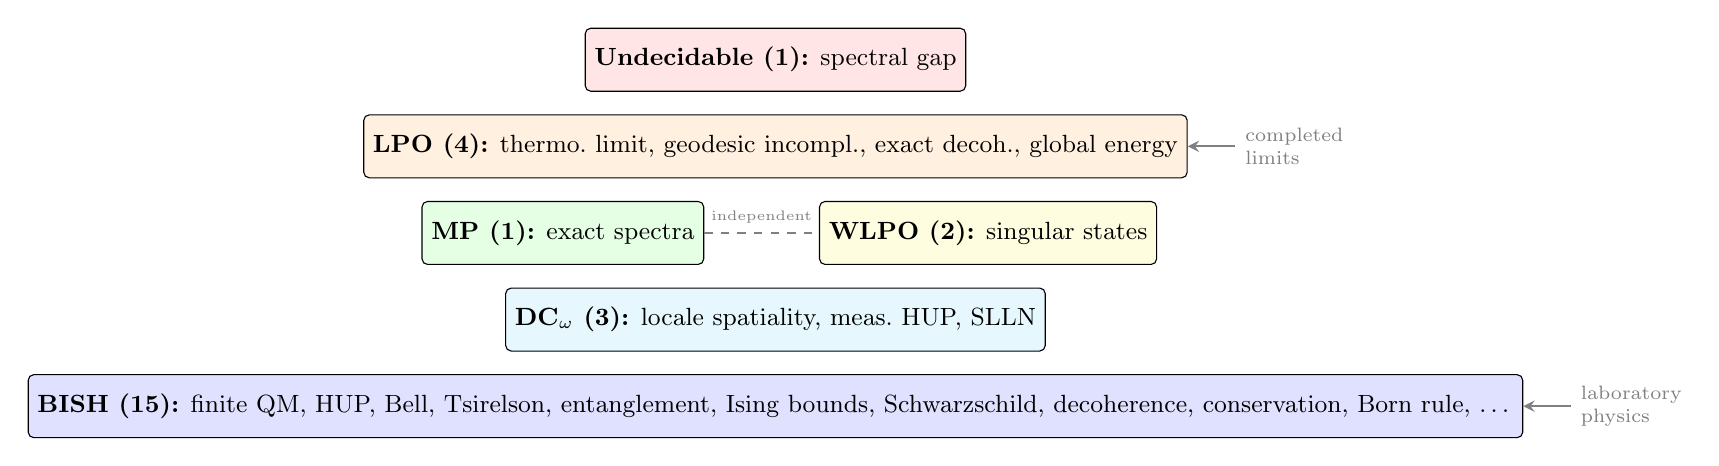
\begin{tikzpicture}[
  level/.style={draw, minimum height=0.8cm, rounded corners=2pt, font=\small,
    align=center},
  >=stealth
]
% Pyramid layers (wider at bottom = more entries at BISH)
\node[level, fill=blue!12, minimum width=12.5cm] (bish) at (0,0)
  {\textbf{BISH (15):} finite QM, HUP, Bell, Tsirelson, entanglement,
   Ising bounds, Schwarzschild, decoherence, conservation, Born rule, \ldots};
\node[level, fill=cyan!10, minimum width=6cm] (dc) at (0,1.1)
  {\textbf{DC$_\omega$ (3):} locale spatiality, meas.\ HUP, SLLN};
\node[level, fill=green!10, minimum width=3.2cm] (mp) at (-2.7,2.2)
  {\textbf{MP (1):} exact spectra};
\node[level, fill=yellow!12, minimum width=3.2cm] (wlpo) at (2.7,2.2)
  {\textbf{WLPO (2):} singular states};
\node[level, fill=orange!12, minimum width=7.5cm] (lpo) at (0,3.3)
  {\textbf{LPO (4):} thermo.\ limit, geodesic incompl., exact decoh., global energy};
\node[level, fill=red!10, minimum width=3cm] (undec) at (0,4.4)
  {\textbf{Undecidable (1):} spectral gap};

% Annotations (anchored to right edges of boxes, not inside them)
\draw[<-, thick, gray] (bish.east) -- +(0.6,0) node[right, font=\scriptsize, gray, align=left] {laboratory\\physics};
\draw[<-, thick, gray] (lpo.east) -- +(0.6,0) node[right, font=\scriptsize, gray, align=left] {completed\\limits};

% Independence annotation for MP/WLPO
\draw[dashed, gray] (mp.east) -- node[above, font=\tiny, gray] {independent} (wlpo.west);

\end{tikzpicture}%
}
\caption{Distribution of calibrated entries across logical levels. The wide BISH base contains all finite-system, finite-time, and finite-sample physics. Non-constructive costs arise only from infinite-limit idealizations (LPO), choice over infinite sequences (DC$_\omega$), or undecidable structural questions. MP and WLPO occupy independent positions in the partial order.}
\label{fig:pyramid}
\end{figure}

\subsection{Why this demands explanation}

One might dismiss the correlation as tautological: of course stronger mathematics is needed for stronger claims. But the correlation is not between logical strength and \emph{mathematical generality} --- it is between logical strength and \emph{physical idealization}. The claims at each level are about the same physical system (say, a quantum spin chain). The difference is how far the mathematical description extends beyond what a laboratory can instantiate.

Finite-volume physics is what we can actually \emph{do}: prepare states, measure observables, record outcomes, all in finite time with finite precision. The WLPO level introduces infinite-dimensional spaces --- Hilbert spaces with countably many degrees of freedom. The LPO level introduces infinite-volume limits --- the fiction that the spin chain extends to infinity. The undecidable level asks questions about those infinite limits that no finite procedure can resolve.

The correlation, then, is between logical strength and \emph{distance from operational reality}. This is a substantive observation, not a tautology. There is no a priori reason why the constructive hierarchy --- which was developed for purely mathematical purposes by Ishihara, Bridges, and others --- should track the layers of physical idealization in this way.

\subsection{Comparison with van Wierst}

Van Wierst [2019] was the first to examine phase transitions through a constructive lens, arguing that constructive mathematics forces ``de-idealizations'' of statistical-mechanical theories: no actual infinities, no discontinuous functions, and constructive real numbers that reflect the imperfect methods by which we determine physical quantities. (Regarding discontinuity: in BISH, WLPO is equivalent to the existence of a discontinuous function in a precise sense [Diener 2018]; absence of WLPO thus blocks one from \emph{proving} such a function exists, though BISH does not positively assert Brouwerian continuity principles.) Van Wierst's argument is primarily philosophical. Our contribution is to supply the precise logical price tags: not merely ``constructive mathematics forces de-idealization,'' but ``the thermodynamic limit costs \emph{exactly} LPO, and the singular-state distinction costs \emph{exactly} WLPO.''

\subsection{Comparison with Batterman}

Batterman [2005, 2011] has argued that infinite idealizations in physics are sometimes ``explanatorily essential'' --- that finite-system descriptions, even when empirically adequate, fail to explain phenomena like universality and renormalization-group fixed points. Our results do not directly contradict Batterman, but they sharpen the debate. Paper~8 shows that for the 1D Ising model, finite-size bounds recover the empirical content of the thermodynamic limit constructively. The question Batterman raises --- whether the \emph{explanatory} content survives --- is not resolved by our formalization, which addresses only the \emph{predictive} content. But the separation between predictive and explanatory content is now formally precise: the predictions are BISH, the explanation (if it requires the completed infinite-volume limit) is LPO. Paper~13 extends this observation to general relativity: the finite-time physics of an infalling observer is BISH, while the singularity assertion as a completed limit costs LPO --- the same logical price as the thermodynamic limit.

\subsection{Comparison with Pour-El and Richards}

Pour-El and Richards [1989] established that even computable initial data can evolve under the wave equation into non-computable solutions --- physical dynamics producing non-computable outputs. Our results address a different layer: even before considering dynamics, the \emph{spaces} in which physics lives have non-computable structure. The trace-class operators require WLPO merely to witness their non-reflexivity; no dynamics are involved. Together, Pour-El-Richards and our results suggest that computability constraints on physics are severe at multiple levels --- both in the state spaces and in the evolution equations.

\section{The Working Hypothesis}

\subsection{Statement}

\textbf{Working Hypothesis (Logical Geography).} In the constructive reverse mathematics of mathematical physics, all non-constructive costs arise from infinite-dimensional idealization layers --- thermodynamic limits, operator completions, bidual passages, singularity assertions as completed limits --- not from the finite-dimensional or finite-time physical content (algebraic relations, symmetries, conservation laws, entanglement structure, cycloid geodesics, curvature scalars). Empirical predictions --- the outputs of physical theories for finite experimental specifications --- are BISH-derivable. Stronger logical principles (DC$_\omega$, MP, WLPO, LPO, LEM) enter the mathematical description of physics only through idealizations that no finite laboratory can instantiate.

The evidence now spans six domains of mathematical physics:
\begin{itemize}
\item \emph{Functional analysis}: bidual gap in $\ell^1$ $\equiv$ WLPO (Paper~2), trace-class non-reflexivity $\equiv$ WLPO (Paper~7).
\item \emph{Statistical mechanics}: thermodynamic limit $\equiv$ LPO (Paper~8), formulation-invariant across transfer-matrix and combinatorial routes (Paper~9).
\item \emph{Quantum information}: Tsirelson bound, Bell state entropy, partial trace = BISH (Paper~11).
\item \emph{General relativity}: Schwarzschild exterior = BISH (Paper~1), interior finite-time physics = BISH (Paper~13), geodesic incompleteness $\equiv$ LPO (Paper~13).
\item \emph{Quantum measurement / decoherence}: finite-step decoherence = BISH, exact decoherence $\equiv$ LPO (Paper~14); Born probabilities, weak law = BISH, strong law $\leq$ DC$_\omega$ (Paper~16).
\item \emph{Conservation laws / field theory}: local conservation (Noether) = BISH, global energy $\equiv$ LPO (Paper~15).
\end{itemize}

\noindent Papers~13, 14, and~15 are especially significant because they demonstrate the BMC~$\equiv$~LPO pattern in four completely independent physical domains (statistical mechanics, general relativity, quantum decoherence, conservation laws), using the same logical equivalence applied to different classes of physically motivated monotone sequences.

This is not operationalism. Operationalism rejects the meaningfulness of claims that transcend operational procedures. We do not reject the thermodynamic limit or singular states as meaningless. We observe that their mathematical formulation requires specific logical principles, and we hypothesize that these principles track the boundary between the physically realizable and the mathematically ideal. The hypothesis is about \emph{logical structure}, not about ontological commitment.

\subsection{Distinguishing features}

The hypothesis makes three claims that go beyond the bare correlation:

First, \emph{completeness}: every empirical prediction of mathematical physics is BISH-derivable. This is not established by our results, which cover functional analysis (Papers~2, 7), statistical mechanics (Papers~8, 9), quantum information (Paper~11), general relativity (Paper~13), quantum decoherence (Paper~14), conservation laws (Paper~15), and quantum measurement statistics (Paper~16). But the consistency of the pattern across six distinct domains strengthens the conjecture.

Second, \emph{monotonicity}: along the omniscience spine, the logical cost increases with the degree of idealization. This is established for the layers we have calibrated, but the claim is that no counterexample exists --- there is no physical prediction that requires LPO but whose underlying system is finite-dimensional, and no idealization that is weaker than singular states but whose logical cost exceeds WLPO. The monotonicity claim applies to the dominant spine (BISH $<$ WLPO $<$ LPO); the orthogonal axes (DC$_\omega$, MP) enrich the landscape without violating it.

Third, \emph{formulation-invariance}: the logical costs are properties of the physics, not of the mathematical formulation. This is the strongest and most testable claim. Paper~9 [Lee 2026e] provides the first positive evidence: the LPO cost of the thermodynamic limit is identical across transfer-matrix and combinatorial formulations. We discuss the scope and limitations of this evidence in \S6.

\subsection{Relation to the Church-Turing thesis}

Our hypothesis stands in a natural relationship to the Church-Turing thesis as a physical principle. Deutsch [1985] proposed that the laws of physics should permit only computations consistent with the Church-Turing thesis (or its quantum generalization). This amounts to requiring that nature implement at most the computable functions.

Our hypothesis is both more and less demanding. It is more demanding in that BISH is stricter than Turing computability: there exist Turing-computable functions that are not constructively definable (because BISH requires \emph{proofs} of totality, not mere algorithms). It is less demanding in that we do not require physical theories to be computable in the Church-Turing sense --- we require only that their empirical content be expressible in BISH, which is a constraint on \emph{logical structure} rather than \emph{algorithmic complexity}.

The relationship to the extended Church-Turing thesis (that no physical process can compute a function not computable by a Turing machine) is also illuminating. If nature operates at BISH, then certainly the extended Church-Turing thesis holds --- but the converse is false. Turing computability plus classical logic gives you more than BISH. Our hypothesis occupies a specific position between the Church-Turing thesis and full classical logic.

\subsection{Subsumption of the digital physics critique}

In a supplementary note [Lee 2026d], we derived a trilemma for digital physics programs: any program claiming the universe is fundamentally computational must either (i) accept finitism (no infinite-dimensional state spaces at all), (ii) accept hypercomputation (a computational universe that somehow transcends Turing limits), or (iii) reconstruct physics constructively to avoid bidual-gap arguments. That trilemma is a corollary of the present hypothesis.

If the hypothesis is correct, horn~(iii) is the natural resolution: the physics \emph{is} reconstructible at the constructive level, because the empirical content never needed the non-constructive superstructure. The bidual gap is real as mathematics (Papers~2 and~7 verify this), but its physical significance is precisely that it marks the boundary beyond which the formalism outruns the physics. A digital physics program that operates at the BISH level --- computing finite-volume predictions with constructive error bounds --- captures everything a laboratory can verify. The infinite-dimensional overhead is the mathematician's convenience, not nature's structure.

\subsection{Relation to Gisin's intuitionistic physics}

Gisin [2020, 2021] has argued philosophically for ``intuitionistic physics'' --- a reformulation of physics avoiding infinite precision and non-constructive existence claims. Gisin's argument is primarily conceptual, motivated by the observation that real numbers with infinite decimal expansions encode more information than any physical measurement can access. He does not provide the technical price tag for his proposal.

Our results supply that price tag. If physics is to be intuitionistic (in the sense of avoiding WLPO), it must abandon or reconstruct: the density-matrix formalism for mixed states (since the normal/singular distinction requires WLPO), the thermodynamic limit for phase transitions (which requires the stronger LPO), singularity assertions in general relativity (which also require LPO), and more broadly, any argument that distinguishes reflexive from non-reflexive spaces. The positive news: quantum entanglement structure (Paper~11) is already intuitionistic, and finite-time gravitational physics (Paper~13) requires no reconstruction. So too are finite-step decoherence bounds (Paper~14), local conservation laws (Paper~15), and Born probabilities and finite-sample error bounds (Paper~16). Whether the full reconstruction is possible while preserving empirical content is the open problem we have identified --- and Paper~8, Part~A provides the first affirmative instance for statistical mechanics, while Paper~13 provides the first instance for general relativity.

\section{The Formulation-Invariance Test}

The hypothesis predicts that the logical costs are properties of the physics, not of the mathematical formulation. Paper~9 [Lee 2026e] provides the first test of this prediction.

\subsection{The test and its outcome}

\textbf{Test.} If the logical cost of the thermodynamic limit is intrinsic to the physics, then mathematically independent derivations of the same physical quantity should yield identical axiom profiles. If the cost is an artifact of the formalism, different formulations should yield different profiles.

\textbf{Outcome.} Paper~9 re-derives both results of Paper~8 --- the BISH dispensability of finite-size bounds (Part~A) and the LPO equivalence of the thermodynamic limit (Part~B) --- using purely combinatorial methods. The partition function identity $Z_N(\beta) = (2\cosh\beta)^N + (2\sinh\beta)^N$ is established via bond variables and the binomial parity sieve, replacing the transfer-matrix spectral decomposition $Z_N = \operatorname{Tr}(T^N) = \lambda_+^N + \lambda_-^N$ entirely. No matrices, eigenvalues, linear algebra, or functional analysis appear at any point.

The formulation-invariance claim is verified at two levels. First, the \emph{axiom audit}: the \texttt{\#print axioms} output for both formalizations is identical --- \texttt{[propext, Classical.choice, Quot.sound]} for Part~A, with the addition of \texttt{bmc\_of\_lpo} for the Part~B equivalence. (The combinatorial formalization also axiomatizes a parity sieve identity --- an elementary combinatorial fact requiring nontrivial Lean infrastructure to formalize; this axiom is architecturally isolated from the main theorem dependency chains and does not appear in the \texttt{\#print axioms} output for either the dispensability or equivalence theorems.) Second, the \emph{import audit}: the combinatorial formalization imports no Mathlib module from \texttt{LinearAlgebra.*} or \texttt{Analysis.NormedSpace.*}, ensuring strict separation from the transfer-matrix approach. The two formalizations share only the unavoidable common substrate --- real arithmetic and the logical principles under test.

The result: two mathematically independent routes to the same physical quantity produce the same logical cost. The LPO-strength of the thermodynamic limit is not an artifact of the transfer-matrix formalism.

\subsection{Scope and limitations}

The formulation-invariance result is evidence, not proof. Two formulations are better than one, but a definitive result would be an \emph{ineliminability} theorem: that \emph{any} constructive proof of free energy convergence for the 1D Ising model must use BMC. This remains an open problem (Problem~1 below).

The test has been carried out only at the LPO level and only for the 1D Ising model. Whether the WLPO cost of the bidual gap (Papers~2, 7) is similarly formulation-invariant --- whether the same logical cost arises in the C*-algebraic formulation as in the Banach-space formulation --- is an open question (Problem~5 below).

\subsection{Domain invariance: Papers 8, 13, 14, and 15}

The formulation-invariance of Papers~8 and~9 concerns a single physical system (the 1D Ising model) described in two mathematical languages. Papers~13, 14, and~15 reveal a different and arguably deeper invariance: \emph{domain invariance}. All four papers use the BMC~$\equiv$~LPO equivalence, but they apply it to unrelated physical systems:

\begin{itemize}
\item Paper~8: coupling constant modulation $\to$ free energy sequence $\to$ BMC.
\item Paper~13: sequence coupling $\to$ infalling proper-time trajectory $\to$ BMC.
\item Paper~14: decoherence angle $\to$ coherence sequence $c(N)$ $\to$ ABC ($\equiv$ BMC via sign-flip).
\item Paper~15: energy densities $\to$ partial energy sums $E_N$ $\to$ NPSC ($\equiv$ BMC via telescoping).
\end{itemize}

\noindent The same logical structure --- bounded monotone convergence as the exact price of asserting a completed limit --- now appears in four independent physical domains: statistical mechanics, general relativity, quantum decoherence, and conservation laws. Papers~14 and~15 each introduce a named equivalence variant (Antitone Bounded Convergence and Nonneg\-ative Partial Sum Convergence, respectively), both of which are fully proved equivalent to BMC in Lean with no custom axioms. The surface mechanism varies across domains --- sign-flip for antitone sequences, telescoping for nonnegative partial sums --- but the underlying logical structure is invariant: BMC~$\equiv$~LPO.

Paper~15 introduces a qualitative novelty: it is the first calibration of a \emph{structural law} (Noether's theorem: symmetry implies conservation) rather than a physical prediction. The LPO cost is not tied to any specific physical system but to the \emph{operation} of summing a nonnegative density to infinity --- a pattern that recurs across all domains where positive-definite quantities are integrated over infinite systems.

This is strong evidence that the calibration is not an artifact of specific encodings or mathematical formulations: the BMC~$\equiv$~LPO cost is intrinsic to the operation of passing from a bounded monotone sequence to its limit, regardless of the physical domain that produces the sequence. Figure~\ref{fig:domain-invariance} displays this structural parallelism.

\begin{figure}[ht]
\centering
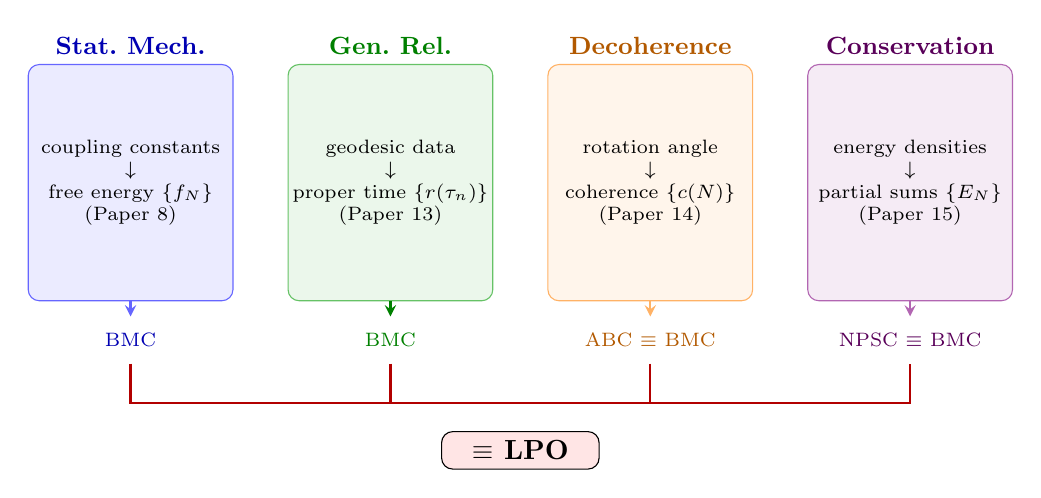
\begin{tikzpicture}[
  pillar/.style={draw, rounded corners, minimum width=2.6cm, minimum height=3cm,
    fill=#1!8, draw=#1!60},
  plabel/.style={font=\small\bfseries, #1},
  >=stealth
]
% Four pillars
\node[pillar=blue] (sm) at (0,0) {};
\node[plabel=blue!70!black, above] at (sm.north) {Stat.\ Mech.};
\node[font=\scriptsize, align=center] at (sm.center) {coupling constants\\$\downarrow$\\free energy $\{f_N\}$\\(Paper~8)};

\node[pillar=green!60!black] (gr) at (3.3,0) {};
\node[plabel=green!50!black, above] at (gr.north) {Gen.\ Rel.};
\node[font=\scriptsize, align=center] at (gr.center) {geodesic data\\$\downarrow$\\proper time $\{r(\tau_n)\}$\\(Paper~13)};

\node[pillar=orange] (dc) at (6.6,0) {};
\node[plabel=orange!70!black, above] at (dc.north) {Decoherence};
\node[font=\scriptsize, align=center] at (dc.center) {rotation angle\\$\downarrow$\\coherence $\{c(N)\}$\\(Paper~14)};

\node[pillar=violet] (cl) at (9.9,0) {};
\node[plabel=violet!70!black, above] at (cl.north) {Conservation};
\node[font=\scriptsize, align=center] at (cl.center) {energy densities\\$\downarrow$\\partial sums $\{E_N\}$\\(Paper~15)};

% Convergence labels below pillars
\node[font=\scriptsize, blue!70!black] at (0,-2) {BMC};
\node[font=\scriptsize, green!50!black] at (3.3,-2) {BMC};
\node[font=\scriptsize, orange!70!black] at (6.6,-2) {ABC $\equiv$ BMC};
\node[font=\scriptsize, violet!70!black] at (9.9,-2) {NPSC $\equiv$ BMC};

% Arrows down from pillars
\draw[->, thick, blue!60] (sm.south) -- (0,-1.7);
\draw[->, thick, green!50!black] (gr.south) -- (3.3,-1.7);
\draw[->, thick, orange!60] (dc.south) -- (6.6,-1.7);
\draw[->, thick, violet!60] (cl.south) -- (9.9,-1.7);

% Connecting arch to LPO
\draw[thick, red!70!black] (0,-2.3) -- (0,-2.8) -- (9.9,-2.8) -- (9.9,-2.3);
\draw[thick, red!70!black] (3.3,-2.3) -- (3.3,-2.8);
\draw[thick, red!70!black] (6.6,-2.3) -- (6.6,-2.8);
\node[draw, rounded corners, fill=red!10, font=\bfseries, minimum width=2cm] at (4.95,-3.4) {$\equiv$ LPO};

\end{tikzpicture}
\caption{Domain invariance of the BMC~$\equiv$~LPO calibration. Four independent physical domains each produce a bounded monotone sequence whose completed-limit existence costs exactly LPO. The surface mechanism varies (sign-flip for ABC, telescoping for NPSC), but the underlying logical structure is invariant.}
\label{fig:domain-invariance}
\end{figure}

\subsection{The encoding objection}

A natural objection to the calibration results is that they depend on encoding: the equivalence between LPO and free energy convergence (Paper~8, Part~B) works by encoding a binary sequence into coupling constants, and the resulting Hamiltonian may be ``artificial.'' If the logical cost is an artifact of the encoding rather than a property of the physics, the calibration is meaningless.

We address this directly. The encoding objection conflates two questions: (i) Is the Hamiltonian physically natural? (ii) Is the logical equivalence informative? For~(i), the encoded Hamiltonian is a legitimate nearest-neighbour 1D Ising model with site-dependent couplings --- unusual in the physics literature, but not artificial in any mathematical sense. For~(ii), the equivalence is informative precisely because it shows that BMC (bounded monotone convergence) is the \emph{exact} logical content of thermodynamic-limit existence for this class of models. The encoding is the proof technique; the calibration is the result.

Moreover, Paper~9 strengthens the response to this objection: the same encoding strategy works in the combinatorial formulation, producing identical axiom profiles. The encoding is not tied to the transfer-matrix framework.

\subsection{The topos-theoretic alternative}

A significant challenge to our hypothesis comes from the D\"oring-Isham topos program [Isham 1997, D\"oring and Isham 2008, Heunen, Landsman, and Spitters 2009]. This program reformulates quantum mechanics within a topos --- a generalized universe of sets with an intuitionistic internal logic. In the topos associated with a von Neumann algebra, the Kochen-Specker theorem is reinterpreted as the non-existence of global sections of a certain presheaf, and quantum states become probability valuations on the spectral presheaf.

The internal logic of these topoi is intuitionistic, hence compatible with constructive mathematics. If the entire empirical content of quantum theory can be recovered within the D\"oring-Isham framework, this would support our hypothesis: the physics would be expressible in an intuitionistic (hence constructive-compatible) framework, with classical logic entering only through the traditional formulation.

Conversely, if the D\"oring-Isham framework provably \emph{cannot} recover certain empirical predictions without additional classical axioms, this would challenge the hypothesis. The precise relationship between the D\"oring-Isham internal logic and the BISH/WLPO/LPO hierarchy has not been worked out. We flag this as a high-priority question for the programme.

\subsection{What a counterexample would look like}

A decisive refutation of the working hypothesis would take the following form: a \emph{finite-system} measurement prediction --- an expectation value, a correlation function, a transition probability for a system specified by a finite-dimensional Hilbert space, rational Hamiltonian coefficients, and rational error tolerance --- whose derivation from first principles essentially requires WLPO (or a stronger principle), with no constructive alternative derivation yielding the same numerical value within the specified tolerance.

We know of no such counterexample. This is weak evidence in favor of the hypothesis, but it is the correct kind of evidence: the hypothesis survives not because it is unfalsifiable, but because no one has found the relevant counterexample. The search for such a counterexample --- or for a proof that none exists --- is the most immediate concrete research question our proposal generates.

\section{Historical Precedents}

The proposal that a mathematical structure might track physical reality rather than merely representing it has significant precedents.

\subsection{Computation as physics}

Before Landauer [1961] and Bennett [1973], computation was a purely mathematical notion. The insight that computation is a physical process --- requiring energy, dissipating heat, occupying time --- transformed information theory and eventually led to quantum computing. Deutsch [1985] sharpened this by proposing that the set of physically computable functions is determined by physics, not mathematics: quantum physics computes different functions than classical physics.

Our proposal extends this one level up. Deutsch asked: what if \emph{computability} is physical? We ask: what if \emph{logical strength} is physical? The constructive hierarchy (BISH, WLPO, LPO, LEM) is to our proposal what the computability hierarchy (finite automata, pushdown automata, Turing machines) was to Deutsch's.

\subsection{Simultaneity and the operational content of mathematics}

Einstein's 1905 analysis of simultaneity is perhaps the deepest precedent. Einstein asked: what physical content does the claim ``two events are simultaneous'' actually carry? The answer --- that simultaneity requires a synchronization procedure, and different procedures yield different answers for different observers --- was a foundational insight that revolutionized physics.

We ask an analogous question: what physical content does the claim ``this state is singular'' (or ``this Banach space is non-reflexive'' or ``this spectral gap is zero'') actually carry? Our formalized results provide a precise answer: these claims carry the logical content of specific omniscience principles. Whether this logical content has physical substance --- whether the universe ``decides'' these questions or whether they are artifacts of the formalism --- is the question our hypothesis addresses.

\subsection{Constructive mathematics as physics}

There is a long tradition of developing constructive mathematics as the natural language for analysis and computation. Bishop [1967] framed constructive analysis with an algorithmic interpretation. Bridges and Richman [1987] systematized the varieties of constructive mathematics. Beeson [1985] developed the metamathematical foundations. Ishihara [2006] initiated the specific program of constructive reverse mathematics. Diener [2018] compiled the most comprehensive survey. Brattka and Gherardi [2009] connected omniscience principles to the Weihrauch lattice, providing a computational counterpart to the logical classification. The mathematical infrastructure for our proposal has been built by these researchers over decades; our contribution is to connect this infrastructure to the physical hierarchy of idealizations.

\section{Open Problems}

We close by listing specific open problems that would advance the programme.

\textbf{Problem~1.} \emph{Ineliminability.} Papers~8 and~9 establish the LPO cost of the thermodynamic limit via two independent formulations. Is this cost \emph{ineliminable} --- must \emph{any} constructive proof of free energy convergence for the 1D Ising model use BMC? A positive answer would upgrade the formulation-invariance evidence of Paper~9 to a genuine theorem. For the 2D Ising model, where the Peierls argument establishes phase coexistence, the question is sharper: if finite-size bounds for the 2D magnetization can be established constructively, the dispensability extends; if not, there is a genuine LPO obstruction at the empirical level, and the hypothesis is under pressure.

\textbf{Problem~2.} \emph{Phase transitions without limits.} Can phase transitions be characterized constructively --- without asserting the existence of the thermodynamic limit --- in a way that preserves the standard phenomenology (critical exponents, universality classes, scaling relations)? Van Wierst [2019] argues that constructive analysis forces ``de-idealizations'' but does not provide a positive reconstruction.

\textbf{Problem~3.} \emph{Intermediate and orthogonal principles.} The calibration table now includes DC$_\omega$ (measurement uncertainty, locale spatiality) and MP (exact spectral membership) alongside the omniscience spine (WLPO, LPO). Several questions arise: (a)~Does any physical idealization have LLPO (the Lesser Limited Principle of Omniscience, strictly weaker than WLPO in the omniscience hierarchy) as its exact logical cost? (b)~Can the DC$_\omega$ costs of Paper~4 (S2) and Paper~6 (HUP-M) be sharpened to exact equivalences rather than upper bounds? (c)~Is the MP cost of exact spectral membership (Paper~4, S1) formulation-invariant --- does the same cost arise in the C*-algebraic spectral theory as in the Hilbert-space formulation?

\textbf{Problem~4.} \emph{D\"oring-Isham calibration.} What is the constructive strength of the D\"oring-Isham topos framework? Specifically, does the internal logic of the Bohrification topos associated with $B(H)$ coincide with BISH, or does it validate additional principles (WLPO, LPO, or fragments thereof)?

\textbf{Problem~5.} \emph{Formulation-invariance for the WLPO level.} The WLPO equivalence (Papers~2, 7) is stated in the Banach-space formulation of quantum mechanics. Does the same logical cost appear in the C*-algebraic formulation? Specifically, does the GNS construction applied to a state on $B(H)$ --- recovering the density matrix from the algebraic state --- require WLPO?

\textbf{Problem~6.} \emph{Beyond statistical mechanics.} Does the calibration pattern extend to quantum field theory? Papers~14 and~15 have extended the pattern to quantum decoherence and conservation laws, but the renormalization group involves infinite-volume limits (LPO-strength) and also ultraviolet limits (requiring different mathematical infrastructure). What are the logical costs of renormalization?

\textbf{Problem~7.} \emph{Infinite-dimensional entanglement entropy.} Paper~11 establishes that finite-dimensional entanglement structure (Tsirelson bound, Bell state entropy, partial trace) is BISH. Does passage to infinite-dimensional entanglement --- von Neumann entropy of partial traces in $S_1(H)$, entanglement measures for infinite-dimensional systems --- introduce new logical costs? Does it inherit the WLPO cost of Paper~7's non-reflexivity for $S_1(H)$?

\textbf{Problem~8.} \emph{Singularity calibration beyond Schwarzschild.} Paper~13 calibrates geodesic incompleteness for the Schwarzschild interior at LPO. Does the full Penrose singularity theorem --- including trapped surfaces, energy conditions, global hyperbolicity --- calibrate above LPO? Does cosmic censorship (universal quantifier over all generic initial data) have a definite logical cost?

\textbf{Problem~9.} \emph{SLLN calibration sharpness.} Paper~16 establishes that the strong law of large numbers (exact frequentist convergence of Born-rule measurement outcomes) requires at most DC$_\omega$. Is DC$_\omega$ \emph{necessary} for the SLLN, or does a weaker principle suffice? A constructive proof of SLLN~$\equiv$~DC$_\omega$ over BISH would convert Paper~16's upper bound into an exact calibration, completing the DC$_\omega$ row of the table.

\section{Conclusion}

The constructive hierarchy of omniscience and choice principles --- a technical apparatus developed for the internal purposes of constructive analysis --- turns out to map onto the layers of physical idealization in mathematical physics with surprising fidelity. Finite physics, preparation uncertainty, quantum entanglement structure, Schwarzschild interior finite-time physics, decoherence bounds, local conservation laws, and Born probabilities are BISH. Measurement uncertainty, spectral locale extraction, and frequentist convergence cost DC$_\omega$. Exact spectral membership costs MP (on an orthogonal axis). The singular sector costs WLPO. The thermodynamic limit, geodesic incompleteness, exact decoherence, and global energy existence cost LPO. The spectral gap is undecidable. Each step away from what a finite laboratory can instantiate requires a precisely calibrated increment of logical strength --- and the landscape admits not just a linear chain but a partial order, with the omniscience spine supplemented by choice and decidability dimensions.

This could be a coincidence. But the correlation is not between logical strength and mathematical complexity --- it is between logical strength and \emph{physical accessibility}. The same BMC~$\equiv$~LPO equivalence now governs completed limits in four independent domains --- statistical mechanics, general relativity, quantum decoherence, and conservation laws --- a domain invariance that substantially strengthens the evidence that the costs are intrinsic to the physics. The simplest explanation is that nature operates at the constructive level, and the non-constructive superstructure of classical mathematical physics, while enormously convenient, tracks the mathematician's idealizations rather than the world's structure.

We have formulated this as a working hypothesis, established a certification methodology with three levels of evidence, carried out formulation-invariance (Paper~9) and domain-invariance (Papers~8, 13, 14, 15) tests, and identified the open problems that would confirm or refute the hypothesis at greater generality. The programme now encompasses eleven companion papers covering the bidual gap (Paper~2), quantum spectra (Paper~4), uncertainty relations (Paper~6), trace-class operators (Paper~7), the thermodynamic limit via two independent formulations (Papers~8, 9), quantum entanglement (Paper~11), Schwarzschild geodesic incompleteness (Paper~13), quantum decoherence (Paper~14), Noether's theorem and conservation laws (Paper~15), and the Born rule (Paper~16). The precision of the calibration, verified in approximately 12,000 lines of Lean~4 --- predominantly CRM over Mathlib, with Paper~4 using the AxCal methodology --- is unprecedented in the philosophy of mathematical physics. Whether the pattern holds as the programme extends to higher dimensions, quantum field theory, and alternative formulations is the question we leave to future work.

\bigskip

\noindent\textbf{Acknowledgments.} The Lean~4 formalizations and \LaTeX{} manuscripts in this programme were developed with substantial assistance from Claude (Opus~4.6), an AI assistant by Anthropic. The author is not a domain expert in constructive mathematics or mathematical physics; the formalization methodology --- iterative proof construction guided by Lean's type-checker and Mathlib's API --- made this programme tractable for a non-specialist. The author gratefully acknowledges the AI assistance, which was indispensable at every stage: proof strategy, Mathlib API navigation, error diagnosis, and manuscript preparation.

\bigskip

\noindent\textbf{Data availability.} All Lean~4 source code is archived at Zenodo. Paper~2: DOI: 10.5281/zenodo.17107493. Paper~3B: DOI: 10.5281/zenodo.17054155. Paper~4: DOI: 10.5281/zenodo.17059483. Paper~6: DOI: 10.5281/zenodo.18519836. Paper~7: DOI: 10.5281/zenodo.18527559. Paper~8: DOI: 10.5281/zenodo.18516813. Paper~9: DOI: 10.5281/zenodo.18517570. Paper~11: DOI: 10.5281/zenodo.18527676. Paper~14: DOI: 10.5281/zenodo.18569068. Paper~15: DOI: 10.5281/zenodo.18572494. Paper~16: DOI: 10.5281/zenodo.18575377.

\bigskip

\begin{thebibliography}{99}

\bibitem{Batterman2005}
Batterman, R.~W. ``Critical phenomena and breaking drops: Infinite idealizations in physics.'' \emph{Studies in History and Philosophy of Modern Physics} 36 (2005): 225--244.

\bibitem{Batterman2011}
Batterman, R.~W. ``Emergence, singularities, and symmetry breaking.'' \emph{Foundations of Physics} 41 (2011): 1031--1050.

\bibitem{Beeson1985}
Beeson, M.~J. \emph{Foundations of Constructive Mathematics}. Springer, Berlin, 1985.

\bibitem{Bennett1973}
Bennett, C.~H. ``Logical reversibility of computation.'' \emph{IBM Journal of Research and Development} 17(6) (1973): 525--532.

\bibitem{Bishop1967}
Bishop, E. \emph{Foundations of Constructive Analysis}. McGraw-Hill, New York, 1967.

\bibitem{BishopBridges1985}
Bishop, E. and Bridges, D. \emph{Constructive Analysis}. Springer, Berlin, 1985.

\bibitem{BrattkaGherardi2009}
Brattka, V. and Gherardi, G. ``Weihrauch degrees, omniscience principles and weak computability.'' In \emph{6th International Conference on Computability and Complexity in Analysis (CCA'09)}, OASIcs vol.~11, pp.~83--94. Schloss Dagstuhl, 2009.

\bibitem{BratteliRobinson1987}
Bratteli, O. and Robinson, D.~W. \emph{Operator Algebras and Quantum Statistical Mechanics}, Vol.~I. 2nd ed. Springer, Berlin, 1987.

\bibitem{BratteliRobinson1997}
Bratteli, O. and Robinson, D.~W. \emph{Operator Algebras and Quantum Statistical Mechanics}, Vol.~II. 2nd ed. Springer, Berlin, 1997.

\bibitem{BridgesRichman1987}
Bridges, D. and Richman, F. \emph{Varieties of Constructive Mathematics}. Cambridge University Press, 1987.

\bibitem{BridgesVita2006}
Bridges, D. and V\^{\i}\c{t}\u{a}, L.~S. \emph{Techniques of Constructive Analysis}. Springer, New York, 2006.

\bibitem{Cubitt2015}
Cubitt, T.~S., Perez-Garcia, D., and Wolf, M.~M. ``Undecidability of the spectral gap.'' \emph{Nature} 528 (2015): 207--211.

\bibitem{Deutsch1985}
Deutsch, D. ``Quantum theory, the Church-Turing principle and the universal quantum computer.'' \emph{Proceedings of the Royal Society of London A} 400 (1985): 97--117.

\bibitem{Diener2018}
Diener, H. ``Constructive reverse mathematics.'' Habilitation thesis, Universit\"at Siegen, 2018.

\bibitem{DoringIsham2008}
D\"oring, A. and Isham, C.~J. ```What is a thing?': Topos theory in the foundations of physics.'' In \emph{New Structures for Physics}, Lecture Notes in Physics 813, Springer, 2008.

\bibitem{Gisin2020}
Gisin, N. ``Mathematical languages shape our understanding of time in physics.'' \emph{Nature Physics} 16 (2020): 114--116.

\bibitem{Gisin2021}
Gisin, N. ``Indeterminism in physics, classical chaos and Bohmian mechanics: Are real numbers really real?'' \emph{Erkenntnis} 86 (2021): 1469--1481.

\bibitem{Haag1996}
Haag, R. \emph{Local Quantum Physics: Fields, Particles, Algebras}. 2nd ed. Springer, Berlin, 1996.

\bibitem{Heunen2009}
Heunen, C., Landsman, N.~P., and Spitters, B. ``A topos for algebraic quantum theory.'' \emph{Communications in Mathematical Physics} 291 (2009): 63--110.

\bibitem{Isham1997}
Isham, C.~J. ``Topos theory and consistent histories: The internal logic of the set of all consistent sets.'' \emph{International Journal of Theoretical Physics} 36 (1997): 785--814.

\bibitem{Ishihara1992}
Ishihara, H. ``Continuity properties in constructive mathematics.'' \emph{Journal of Symbolic Logic} 57 (1992): 557--565.

\bibitem{Ishihara2006}
Ishihara, H. ``Reverse mathematics in Bishop's constructive mathematics.'' \emph{Philosophia Scientiae}, Cahier sp\'ecial 6 (2006): 43--59.

\bibitem{KadisonRingrose1983}
Kadison, R.~V. and Ringrose, J.~R. \emph{Fundamentals of the Theory of Operator Algebras}, Vol.~I. Academic Press, New York, 1983.

\bibitem{Landauer1961}
Landauer, R. ``Irreversibility and heat generation in the computing process.'' \emph{IBM Journal of Research and Development} 5(3) (1961): 183--191.

\bibitem{Landsman2017}
Landsman, N.~P. \emph{Foundations of Quantum Theory: From Classical Concepts to Operator Algebras}. Springer, 2017.

\bibitem{Lee2026a}
Lee, P.~C.-K. ``Constructive reverse mathematics of the bidual gap: WLPO equivalence for Banach space non-reflexivity.'' 2026a. Lean~4 formalization archived at Zenodo. DOI: 10.5281/zenodo.17107493.

\bibitem{Lee2026b}
Lee, P.~C.-K. ``The physical bidual gap: WLPO and non-reflexivity of trace-class operators.'' 2026b. Lean~4 formalization archived at Zenodo. DOI: 10.5281/zenodo.18527559.

\bibitem{Lee2026c}
Lee, P.~C.-K. ``The constructive cost of the thermodynamic limit: LPO equivalence and BISH dispensability in the 1D Ising model.'' 2026c. Lean~4 formalization archived at Zenodo. DOI: 10.5281/zenodo.18516813.

\bibitem{Lee2026d}
Lee, P.~C.-K. ``Digital physics and the bidual gap: Why computational universes cannot verify Banach space non-reflexivity.'' Supplementary note, 2026d. Available at ResearchGate.

\bibitem{Lee2026e}
Lee, P.~C.-K. ``Formulation-invariance of the logical cost of the thermodynamic limit: A combinatorial proof for the 1D Ising model.'' 2026e. Lean~4 formalization archived at Zenodo. DOI: 10.5281/zenodo.18517570.

\bibitem{Lee2026f}
Lee, P.~C.-K. ``Axiom calibration for quantum spectra: Orthogonal heights, choice principles, and separation portals.'' 2026f. Lean~4 formalization archived at Zenodo. DOI: 10.5281/zenodo.17059483.

\bibitem{Lee2026g}
Lee, P.~C.-K. ``Constructive reverse mathematics for the Heisenberg uncertainty principle: Robertson--Schr\"odinger and Schr\"odinger inequalities over Mathlib.'' 2026g. Lean~4 formalization archived at Zenodo. DOI: 10.5281/zenodo.18519836. (Paper~6, v2; supersedes v1 at DOI: 10.5281/zenodo.17068179.)

\bibitem{Lee2026h}
Lee, P.~C.-K. ``The constructive cost of quantum entanglement: Tsirelson bound and Bell state entropy in Lean~4.'' 2026h. Lean~4 formalization archived at Zenodo. DOI: 10.5281/zenodo.18527676.

\bibitem{Lee2026i}
Lee, P.~C.-K. ``The event horizon as a logical boundary: Schwarzschild interior geodesic incompleteness and LPO in Lean~4.'' 2026i. Lean~4 formalization archived at Zenodo. Paper~13 in the CRM series.

\bibitem{Lee2026j}
Lee, P.~C.-K. ``The measurement problem as a logical artefact: constructive calibration of quantum decoherence.'' 2026j. Lean~4 formalization archived at Zenodo. DOI: 10.5281/zenodo.18569068. Paper~14 in the CRM series.

\bibitem{Lee2026k}
Lee, P.~C.-K. ``Noether's theorem and the logical cost of global conservation laws.'' 2026k. Lean~4 formalization archived at Zenodo. DOI: 10.5281/zenodo.18572494. Paper~15 in the CRM series.

\bibitem{Lee2026l}
Lee, P.~C.-K. ``The Born rule as a logical artefact.'' Technical Note~16. 2026l. Lean~4 formalization archived at Zenodo. DOI: 10.5281/zenodo.18575377. Paper~16 in the CRM series.

\bibitem{PourElRichards1989}
Pour-El, M.~B. and Richards, J.~I. \emph{Computability in Analysis and Physics}. Springer, Berlin, 1989.

\bibitem{Simpson2009}
Simpson, S.~G. \emph{Subsystems of Second Order Arithmetic}. 2nd ed. Cambridge University Press, 2009.

\bibitem{Takesaki1979}
Takesaki, M. \emph{Theory of Operator Algebras I}. Springer, New York, 1979.

\bibitem{vanWierst2019}
van Wierst, P. ``The paradox of phase transitions in the light of constructive mathematics.'' \emph{Synthese} 196 (2019): 1863--1884.

\end{thebibliography}

\end{document}
